\section{Forsøg - Lydens Hastighed}
\subsection{Formål}
Formålet ved dette forsøg er at bestemme lydens hastighed ved hjælp af 2 computere og deres mikrofoner.

\subsection{Udstyr}
\begin{itemize}
    \item 2 computere med programmet audacity
    \item 2 Personer til at klappe
    \item Målebånd til at måde distance
\end{itemize}

\subsection{Fremgangsmåde}
\begin{figure}[h!]
    \centering
    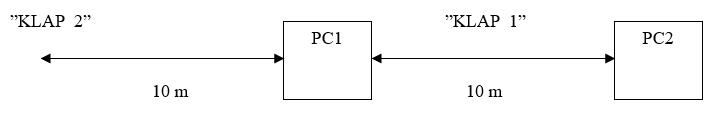
\includegraphics[width=0.7\textwidth]{figures/lydenshastighedforsog.png}
    \caption{Lydens hastighed forsøg}
\end{figure}
\begin{enumerate}
    \item Først skal du placere dine 2 computere så mikrofonerne er 10m fra hinanden.
    \item Start en lydoptagelse ved hjælp af audacity.
    \item Lav et kontrol klap i midten af de 2 computere da de kommer til at få lyden på samme tid.
    \item Efter kontrol klappet skal der klappes igen 10 meter væk fra en af computerene i en ret linje.
    \item Efter det 2. klap skal du afllæse tidsforskellen mellem det første og andet klap.
    \item Tidsforskellen på PC2 minus tidsforskellen på PC1 giver dig tidsforskellen mellem dine klap som du kan bruge til at beregne hastigheden.
\end{enumerate}

\subsection{Resultater}
Vi havde ikke plads til at stå med 10 meters mellemrum, derfor valgte vi at stå med 5 meters mellemrum i stedet.\newline
Tiden det tog lyden at nå computerne var
\begin{itemize}
    \item PC1: 0,852744 sekunder
    \item PC2: 0,867936 sekunder
\end{itemize}
Der giver os en forskel på \begin{math}0,867936s - 0,852744s = 0,15192s\end{math}

\subsection{Resultatbehandling}
For at vide om vores resultat var tæt på den rigtige værdi kan vi bruge formlen for at beregne lydens hastighed ved en bestemt temperatur da lyden er temperaturafhængig.
\begin{equation*}
    v_{lyd} = 331 \cdot \sqrt{\frac{T}{273 K}}  m/s
\end{equation*}
Temperaturen skal være i kelvin. Da vi tog forsøget var der en lufttemperatur på 19C som svarer til \begin{math}19C + 273K = 292K\end{math}
\begin{equation*}
    v_{lyd} = 331 \cdot \sqrt{\frac{292}{273 K}} 342,33 m/s
\end{equation*}

Nu når vi ved hvad hastigheden burde være kan vi beregne hvad vi fik lydens hastighed til, med en formel for hastighed.
\begin{equation*}
    hastighed = \frac{\text{strækning}}{tid} eller v = \frac{s}{t}
\end{equation*}
\begin{equation*}
    v = \frac{5m}{0,015192s} = 329,12 m/s
\end{equation*}